\clearpage
\newpage
\section{Formal Analysis Using Alloy}
\label{sec:Alloy}


\begin{figure}[htbp!]
    \centering
    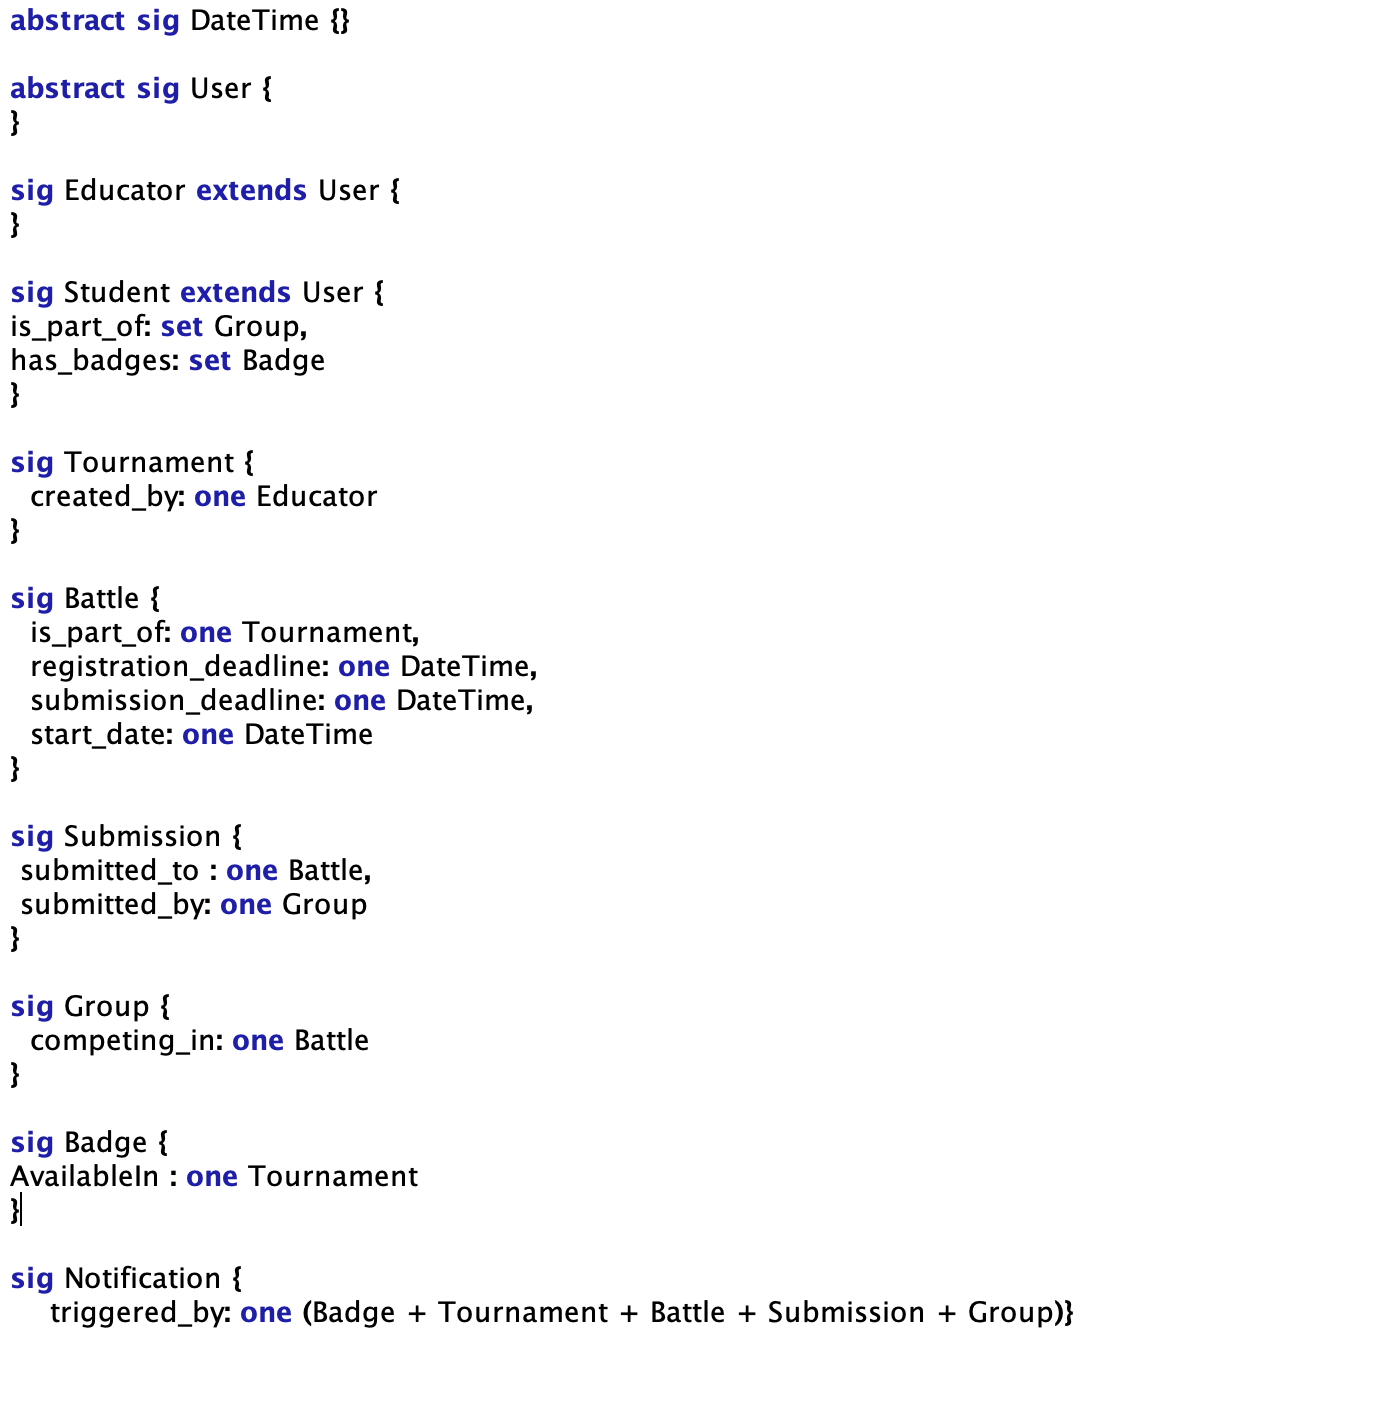
\includegraphics[width=\textwidth]{Graphics/Alloy/Sigs.png}
    \caption{Sigs}
    \label{fig:sigs}
\end{figure}

\begin{figure}[htbp!]
    \centering
    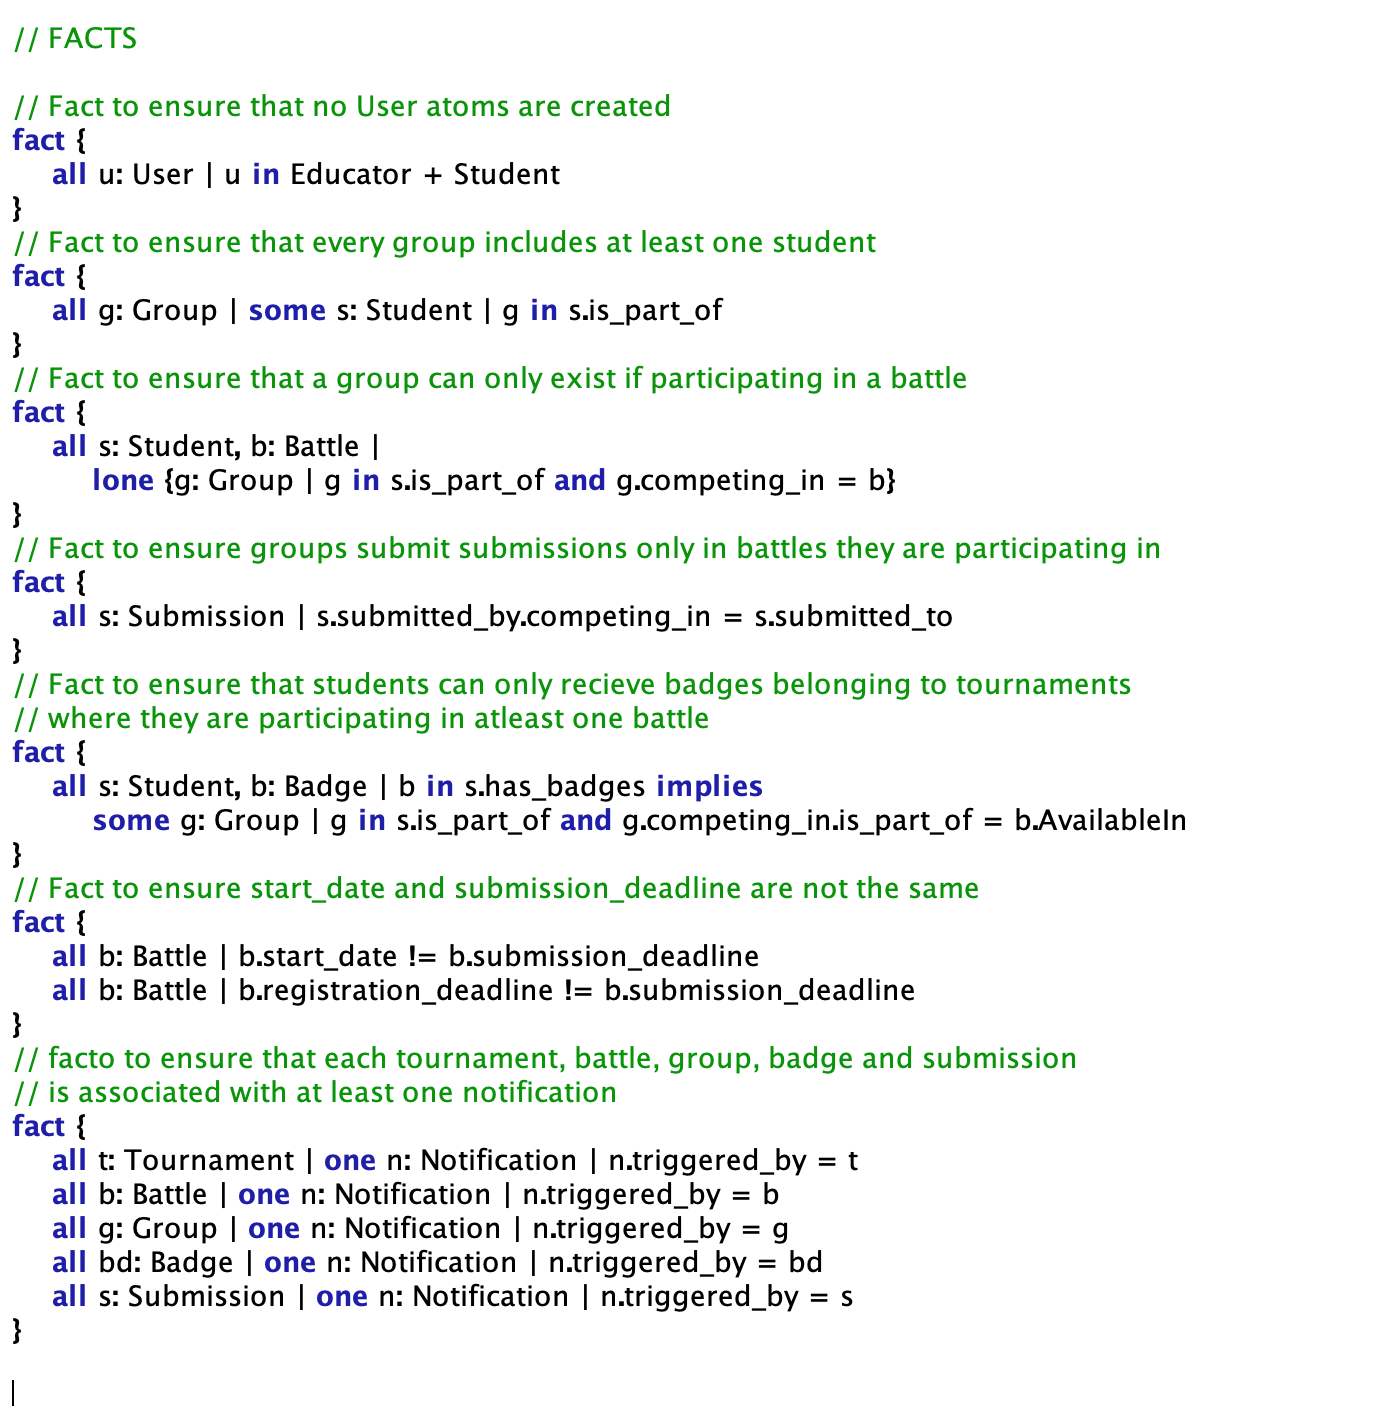
\includegraphics[width=\textwidth]{Graphics/Alloy/Facts.png}
    \caption{Facts}
    \label{fig:Facts}
\end{figure}


\begin{figure}[htbp!]
    \centering
    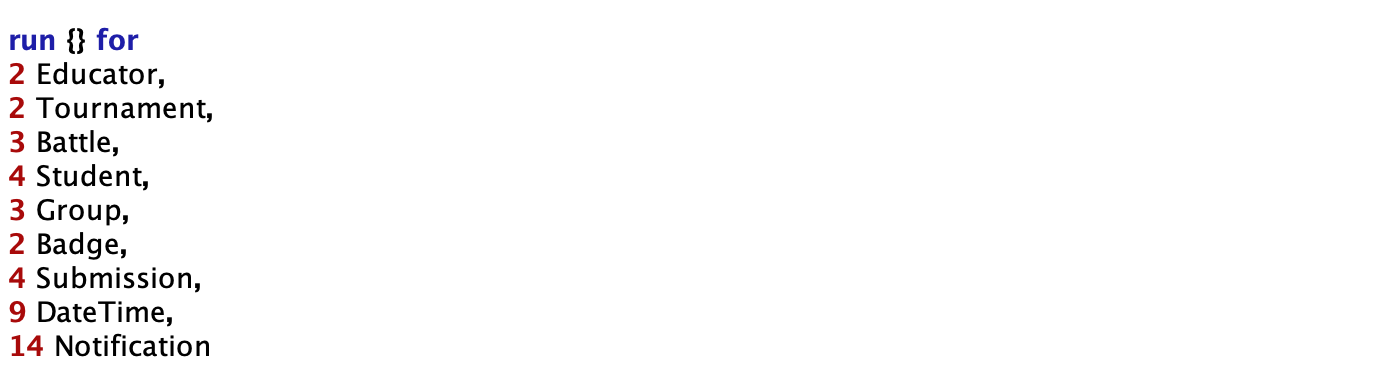
\includegraphics[width=\textwidth]{Graphics/Alloy/Run.png}
    \caption{Run Command}
    \label{fig:runcommand}
\end{figure}


\begin{figure}[htbp!]
    \centering
    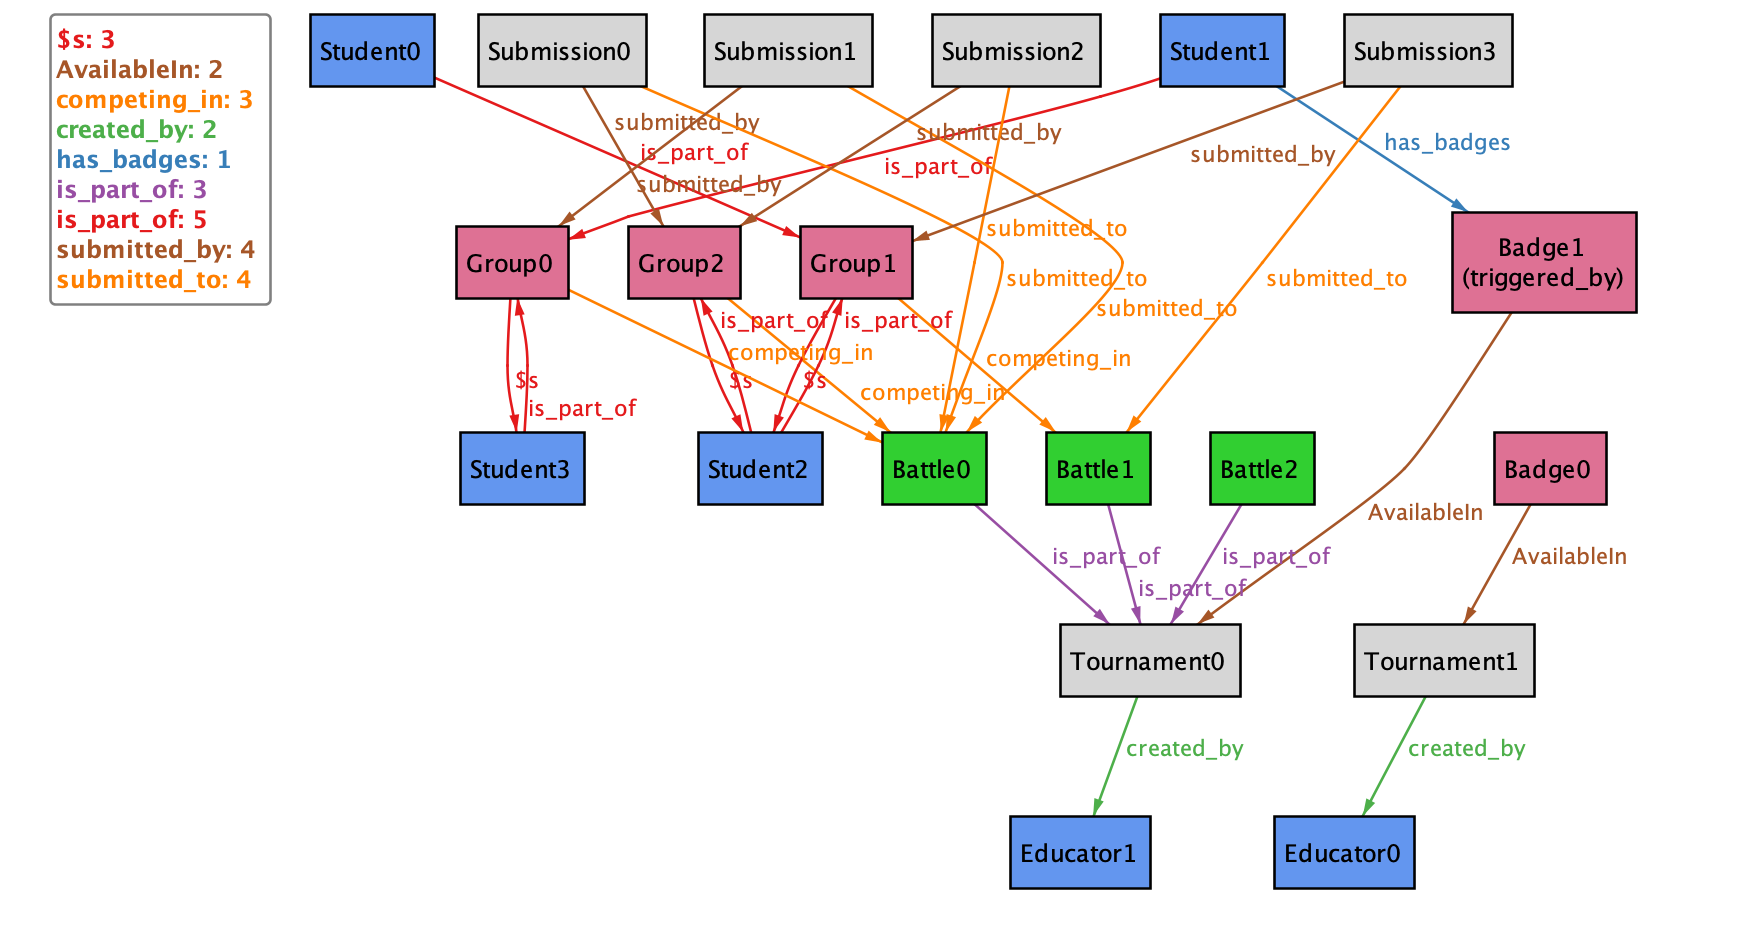
\includegraphics[width=\textwidth]{Graphics/Alloy/Alloy.png}
    \caption{Example}
    \label{fig:example}
\end{figure}

\newpage